\documentclass{article}
\usepackage{amsmath, amsthm, amssymb, booktabs, hyperref, graphicx, float, esint, xcolor, subcaption, csvsimple}
\usepackage[margin=0.5in]{geometry}
\setlength{\abovedisplayskip}{0pt}
\setlength{\belowdisplayskip}{0pt}
\setlength{\abovedisplayshortskip}{0pt}
\setlength{\belowdisplayshortskip}{0pt}

\newcommand{\vr}{\vec{r}}
\newcommand{\vOmega}{\vec{\Omega}}
\newcommand{\vO}{\vec{\Omega}}
\newcommand{\bra}{\left\langle}
\newcommand{\ket}{\right\rangle}
\newcommand{\vdiv}{\vec{\nabla} \cdot}
\newcommand{\vgrad}{\vec{\nabla}}
\newcommand{\vbeta}{\vec{\beta} }
\newcommand{\pdx}{\frac{\partial}{\partial x}}
\newcommand{\pdy}{\frac{\partial}{\partial y}}
\newcommand{\pdz}{\frac{\partial}{\partial z}}
\newcommand{\intrrr}{\int d^3 r \,}
\newcommand{\intrr}{\int d^2 r \,}

\begin{document}
\begin{center}
Ian Halvic \\
\end{center}

%%%%%%%%%%%%%%%%%%%%%%%%%%%%%%%%%%%%%%%%%%%%%%%%%%%%%%%%%%%%%%%%%%%%%%%%%%%%%%%%%%%%%%%%%%%%%%%%%%%%%%
%%%%%%%%%%%%%%%%%%%%%%%%%%%%%%%%%%%%%%%%%%%%%%%%%%%%%%%%%%%%%%%%%%%%%%%%%%%%%%%%%%%%%%%%%%%%%%%%%%%%%%
\section{VEF Sensitivity}
%%%%%%%%%%%%%%%%%%%%%%%%%%%%%%%%%%%%%%%%%%%%%%%%%%%%%%%%%%%%%%%%%%%%%%%%%%%%%%%%%%%%%%%%%%%%%%%%%%%%%%
%%%%%%%%%%%%%%%%%%%%%%%%%%%%%%%%%%%%%%%%%%%%%%%%%%%%%%%%%%%%%%%%%%%%%%%%%%%%%%%%%%%%%%%%%%%%%%%%%%%%%%
For our VEF formulation, the change in QoI approximated to the first order using the adjoint method, while also assuming the Eddington tensor remains remains unperturbed is 
\begin{align*}
\delta QoI =& \bra \phi^\dag , \delta q_0 - \delta \sigma_r \phi + \vdiv \left( \delta c \vdiv \left( E \phi \right) \right)  \ket - \int d^2 r \, \left( E \delta \phi \cdot \left( \frac{1}{ \sigma_{tr}} \left(  \vgrad \phi^\dag \right) \right)^T \right) \cdot \vec{n} \\
&+ \int d^2 r \, \phi^\dag \left[ \left( \frac{1}{\sigma_{tr}} \vdiv \left( E \delta \phi \right) \right) \cdot \vec{n} \right].
\end{align*}
where $\delta c = \frac{1}{\sigma_t + \delta \sigma_t} -  \frac{1}{\sigma_t}$.
Let us focus on the volumetric term due to perturbations in $\sigma_t$
\[
\bra \phi^\dag ,  \vdiv \left( \delta c \vdiv \left( E \phi \right) \right)  \ket
\]
since this is the term (or related to the terms) which are affected by our assumption that the Eddington tensor remains unperturbed.
\subsection{Considering a $\delta E$}
If we were to consider a $\delta E = E_{pert} - E$, then our 1st order approximation would pick up an additional volumetric term (while also creating 2 additional 2nd order terms and a 3rd order perturbation term). Ignoring the boundary terms, the inner product would then be
\[
\delta QoI = \bra \phi^\dag , \delta q_0 - \delta \sigma_r \phi + \vdiv \left( \delta c \vdiv \left( E \phi \right) \right) + \vdiv \left( c \vdiv \left( \delta E \phi \right) \right)  \ket
\]
AN important take away is that this term is scaled with $c$, remembering $c=1/\sigma_t$, low cross-section regions (streaming) has the potential to make "ignoring" this term very costly.

However, a saving grace MAY be present by way of the divergence operators. Green's identity applied to this term yields
\[
\bra \phi^\dag , \vdiv \left( c \vdiv \left( \delta E \phi \right) \right)  \ket 
= 
\bra -\vgrad \phi^\dag , c \vdiv \left( \delta E \phi \right)  \ket + \int_{\delta V} d^2 r \, \phi^\dag  c \vdiv \left( \delta E \phi \right)
\]
So, if in this streaming region, the adjoint is constant constant we would have $\vgrad \phi^\dag =0$, and the volumetric term disappears, and we can focus on the boundaries of the streaming region. [I think this may cause some unpleasant things to happen when we make the jump from 1D slab geometry to 2D and 3D geometries, where the scalar flux has geometric dependence in streaming regions.]


%%%%%%%%%%%%%%%%%%%%%%%%%%%%%%%%%%%%%%%%%%%%%%%%%%%%%%%%%%%%%%%%%%%%%%%%%%%%%%%%%%%%%%%%%%%%%%%%%%%%%%
%%%%%%%%%%%%%%%%%%%%%%%%%%%%%%%%%%%%%%%%%%%%%%%%%%%%%%%%%%%%%%%%%%%%%%%%%%%%%%%%%%%%%%%%%%%%%%%%%%%%%%
\section{Matlab output file format}
%%%%%%%%%%%%%%%%%%%%%%%%%%%%%%%%%%%%%%%%%%%%%%%%%%%%%%%%%%%%%%%%%%%%%%%%%%%%%%%%%%%%%%%%%%%%%%%%%%%%%%
%%%%%%%%%%%%%%%%%%%%%%%%%%%%%%%%%%%%%%%%%%%%%%%%%%%%%%%%%%%%%%%%%%%%%%%%%%%%%%%%%%%%%%%%%%%%%%%%%%%%%%
The Matlab routine sn1d$\_$iterator.m first runs the unperturbed scenario, then runs over various perturbation problems. Data is outputted as a CVS file. The full CSV file has 14 columns, which are
\begin{align*}
Column A &= \text{Problem ID} \\
Column B &= \text{Unperturbed QoI from forward SN} \\
Column C &= \text{Unperturbed QoI from forward VEF} \\
Column D &= \text{Unperturbed QoI from adjoint SN}  \\
Column E &= \text{Unperturbed QoI from adjoint VEF}  \\
Column F &= \delta \sigma_t\text{ factor [0.1 = +\%10]} \\
Column G &= \delta \sigma_s\text{ factor} \\
Column H &= \delta q\text{ factor}  \\
Column I &= \delta \psi_{inc}\text{ factor} \\
Column J &= \delta QoI \text{ Using 2 forward SN solves} \\
Column K &= \delta QoI \text{ Using 2 forward VEF solves} \\
Column L &= \delta QoI \text{ Using SN Adjoint Method} \\
Column M &= \delta QoI \text{ Using VEF Adjoint Method}\\
Column N &= \text{Eddington Error (relative L2)} \\
\end{align*}
In it's current form, the routine only does a single problem at a time, with just a single set of forward solves, so columns A-E will be the same for all lines in the output.
%%%%%%%%%%%%%%%%%%%%%%%%%%%%%%%%%%%%%%%%%%%%%%%%%%%%%%%%%%%%%%%%%%%%%%%%%%%%%%%%%%%%%%%%%%%%%%%%%%%%%%
%%%%%%%%%%%%%%%%%%%%%%%%%%%%%%%%%%%%%%%%%%%%%%%%%%%%%%%%%%%%%%%%%%%%%%%%%%%%%%%%%%%%%%%%%%%%%%%%%%%%%%
\section{Test cases}
%%%%%%%%%%%%%%%%%%%%%%%%%%%%%%%%%%%%%%%%%%%%%%%%%%%%%%%%%%%%%%%%%%%%%%%%%%%%%%%%%%%%%%%%%%%%%%%%%%%%%%
%%%%%%%%%%%%%%%%%%%%%%%%%%%%%%%%%%%%%%%%%%%%%%%%%%%%%%%%%%%%%%%%%%%%%%%%%%%%%%%%%%%%%%%%%%%%%%%%%%%%%%
\subsection{Case \#19 In load\_input.m}
\subsubsection{Overview}
Homogeneous region with homogeneous source. No incident flux from either side. Response is sum of flux in middle $1/5$th of region. Region split into 5 zones, each with a width of 2, 40 elements per zone. $\sigma_t = 2$ and $\sigma_s=1$ for all zones. $\sigma_t$ perturbed uniformly in all zones.

\begin{figure}[H]
\centering
\begin{subfigure}{.5\textwidth}
  \centering
  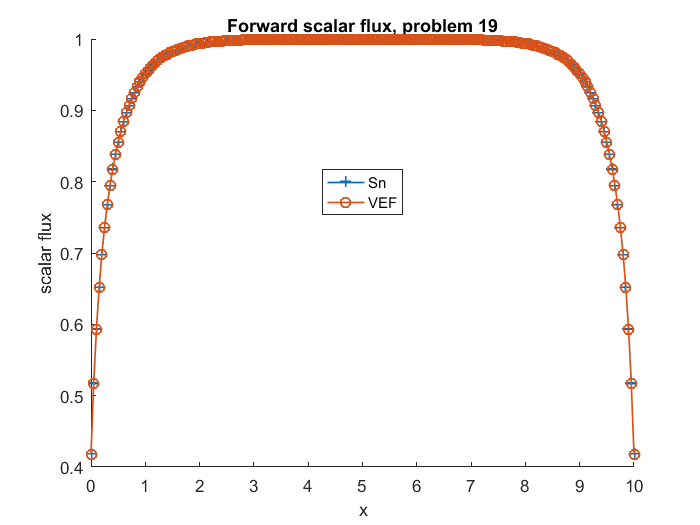
\includegraphics[width=1\linewidth]{p19f.png}
  \caption{Forward}
  \label{fig:sub1}
\end{subfigure}%
\begin{subfigure}{.5\textwidth}
  \centering
  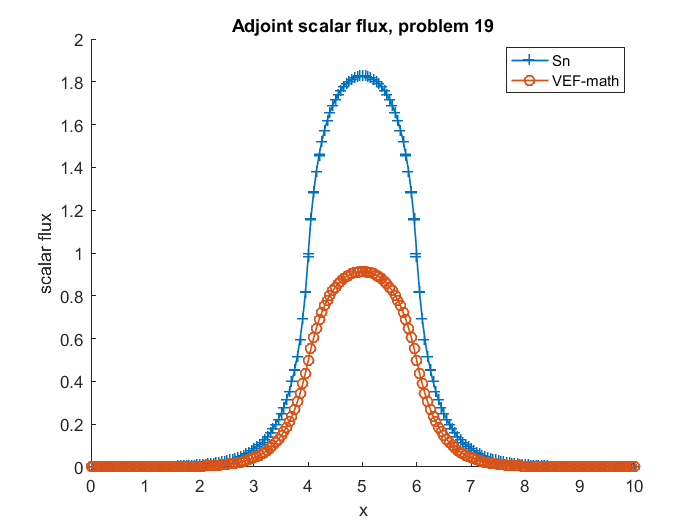
\includegraphics[width=1\linewidth]{p19a.png}
  \caption{Adjoint}
  \label{fig:sub2}
\end{subfigure}
\caption{Unperturbed forward and adjoint solutions for problem 19}
\label{fig:test}
\end{figure}

\subsubsection{Eddington tensor difference}
Below is a graph of the difference in the perturbed and unperturbed Eddington tensor.
\begin{figure}[H]
\centering
\begin{subfigure}{.5\textwidth}
  \centering
  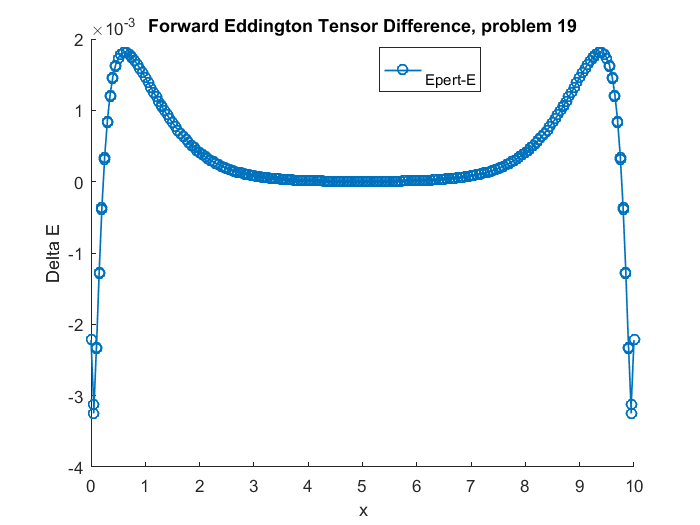
\includegraphics[width=1\linewidth]{p19deltaE.png}
  \caption{$+10\%$ $\sigma_t$. $E_{err}=0.001631$}
  \label{fig:sub1}
\end{subfigure}%
\begin{subfigure}{.5\textwidth}
  \centering
  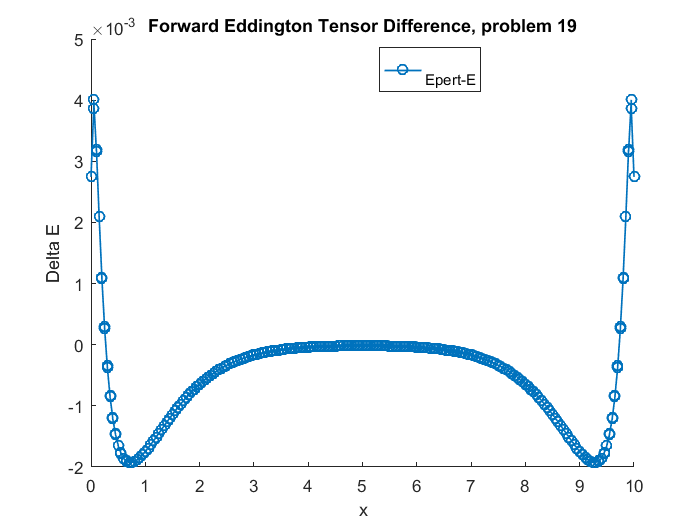
\includegraphics[width=1\linewidth]{p19deltaEdst-10.png}
  \caption{$-10\%$ $\sigma_t$. $E_{err}=0.002052$}
  \label{fig:sub2}
\end{subfigure}
\caption{Eddington difference for $\pm10\%$ $\sigma_t$ for problem 19.}
\label{fig:test}
\end{figure}

\begin{figure}[H]
\centering
\begin{subfigure}{.5\textwidth}
  \centering
  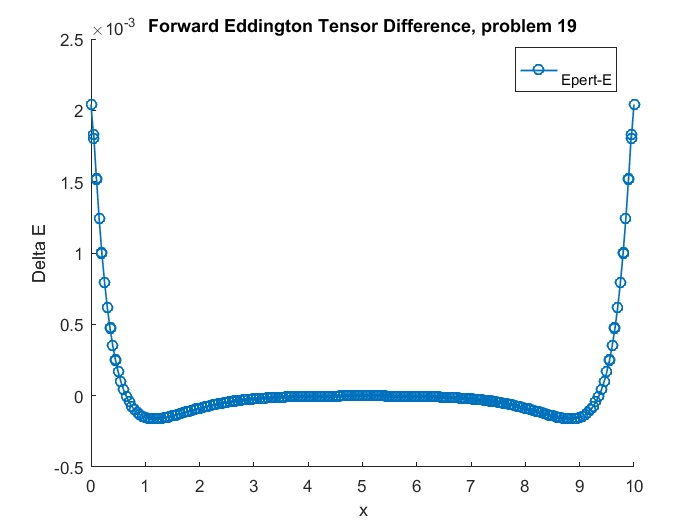
\includegraphics[width=1\linewidth]{p19deltaEdss10.png}
  \caption{$+10\%$ $\sigma_s$. $E_{err}=$}
  \label{fig:sub1}
\end{subfigure}%
\begin{subfigure}{.5\textwidth}
  \centering
  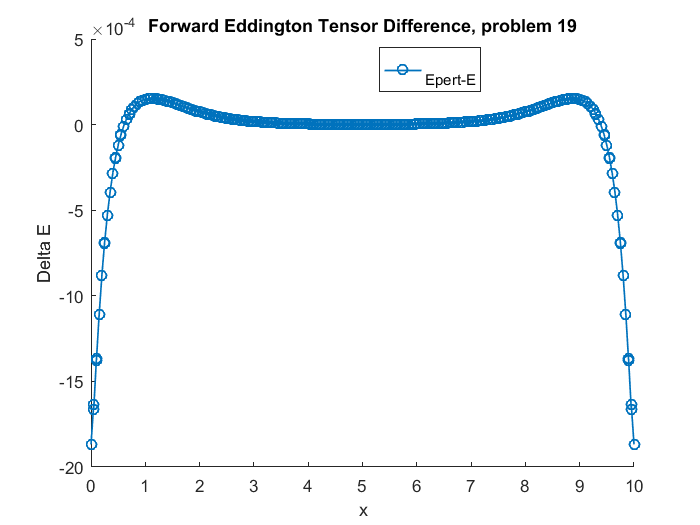
\includegraphics[width=1\linewidth]{p19deltaEdss-10.png}
  \caption{$-10\%$ $\sigma_s$. $E_{err}=$}
  \label{fig:sub2}
\end{subfigure}
\caption{Eddington difference for $\pm10\%$ $\sigma_s$ for problem 19.}
\label{fig:test}
\end{figure}

\begin{figure}[H]
\centering
\begin{subfigure}{.5\textwidth}
  \centering
  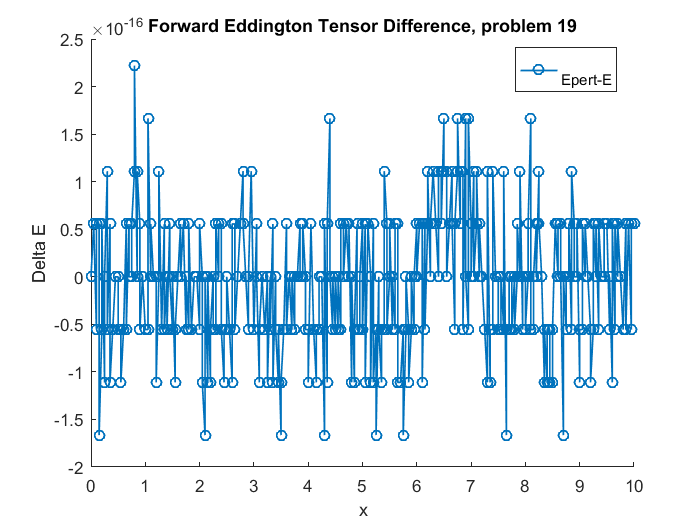
\includegraphics[width=1\linewidth]{p19deltaEdq.png}
  \caption{$+10\%$ $q$. $E_{err}=1.317E-16$}
  \label{fig:sub1}
\end{subfigure}%
\begin{subfigure}{.5\textwidth}
  \centering
  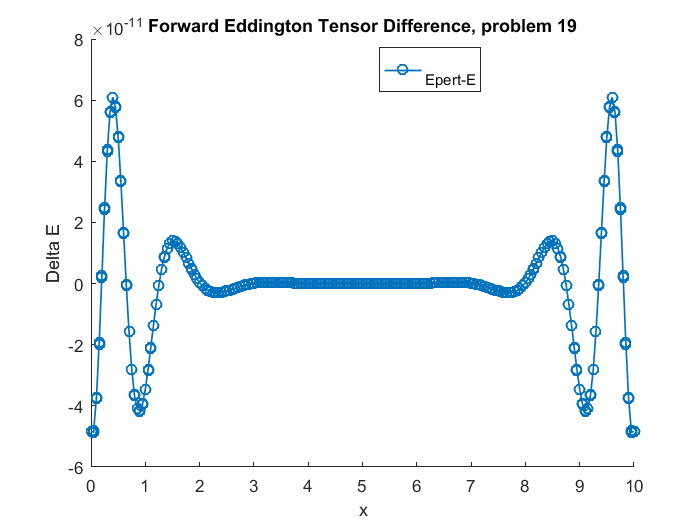
\includegraphics[width=1\linewidth]{p19deltaEdq-10.png}
  \caption{$-10\%$ $q$. $E_{err}=2.864E-11$}
  \label{fig:sub2}
\end{subfigure}
\caption{Eddington difference for $\pm10\%$ $q$ for problem 19.}
\label{fig:test}
\end{figure}

\begin{figure}[H]
\centering
\begin{subfigure}{.5\textwidth}
  \centering
  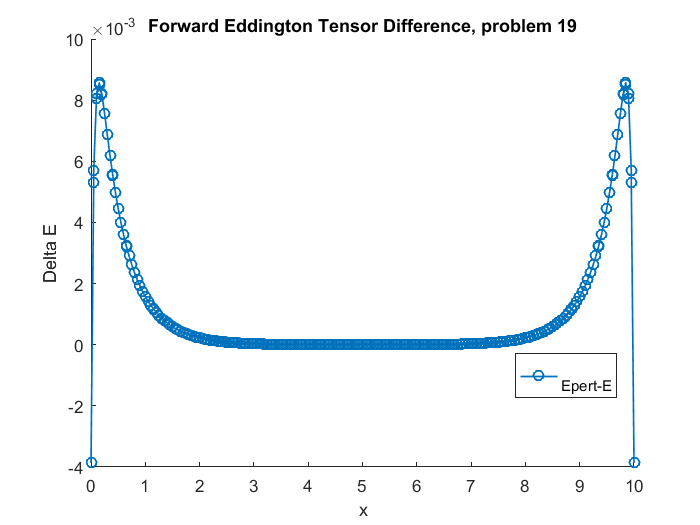
\includegraphics[width=1\linewidth]{p19deltaEdBC0,1.png}
  \caption{$\delta\psi_{inc}=+0.1$. $E_{err}$=$0.001631$}
  \label{fig:sub1}
\end{subfigure}%
\begin{subfigure}{.5\textwidth}
  \centering
  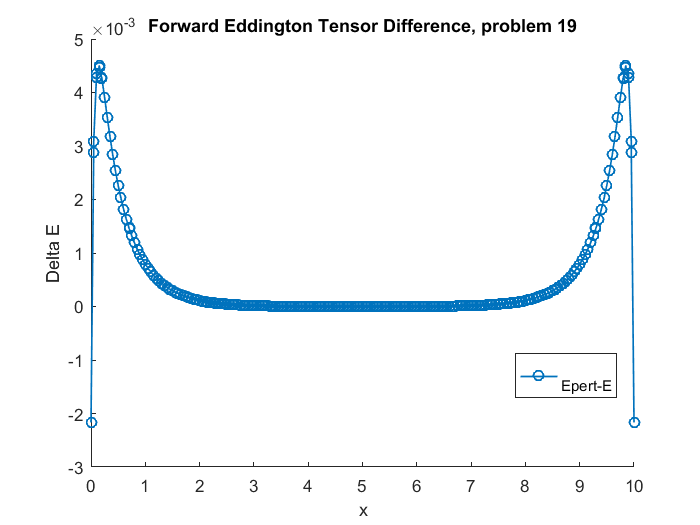
\includegraphics[width=1\linewidth]{p19deltaEdBC0,5.png}
  \caption{$\delta\psi_{inc}=+0.5$. $E_{err}$= $0.002052$}
  \label{fig:sub2}
\end{subfigure}
\caption{Eddington difference for $\psi_{inc}$ perturbations for problem 19.}
\label{fig:test}
\end{figure}


\subsubsection{Perturbation Data Prob 19}
\csvautotabular{DGFEM1D_prob19_short_dst.csv}
\\ \\
\csvautotabular{DGFEM1D_prob19_short_dss.csv}
\\ \\
\csvautotabular{DGFEM1D_prob19_short_dq.csv}
\\ \\
\csvautotabular{DGFEM1D_prob19_short_dBC.csv}

%%%%%%%%%%%%%%%%%%%%%%%%%%%%%%%%%%%%%%%%%%%%%%%%%%%%%%
%%%%%%%%%%%%%%%%%%%%%%%%%%%%%%%%%%%%%%%%%%%%%%%%%%%%%%
\subsection{Case \#20 In load\_input.m}
\subsubsection{Overview}
Nearly identical to case $\#19$, but with an increased mean free path. Homogeneous region with homogeneous source. No incident flux from either side. Response is sum of flux in middle $1/5$th of region. Region split into 5 zones, each with a width of 2, 40 elements per zone. $\sigma_t = 1$ and $\sigma_s=1/2$ for all zones. $\sigma_t$ perturbed uniformly in all zones.

\begin{figure}[H]
\centering
\begin{subfigure}{.5\textwidth}
  \centering
  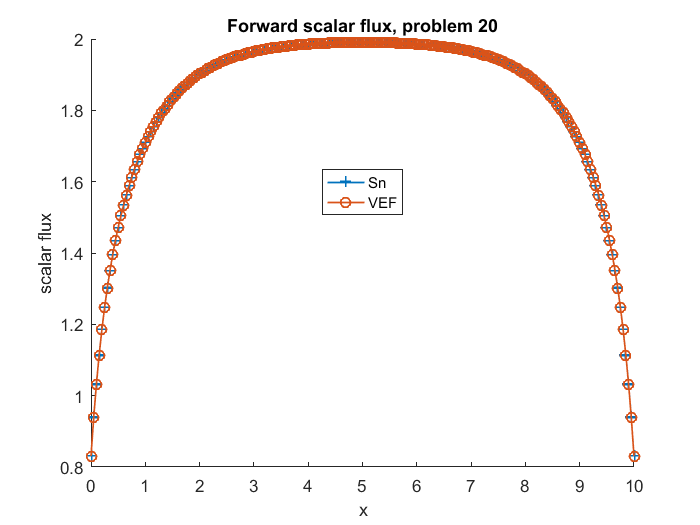
\includegraphics[width=1\linewidth]{p20f.png}
  \caption{Forward}
  \label{fig:sub1}
\end{subfigure}%
\begin{subfigure}{.5\textwidth}
  \centering
  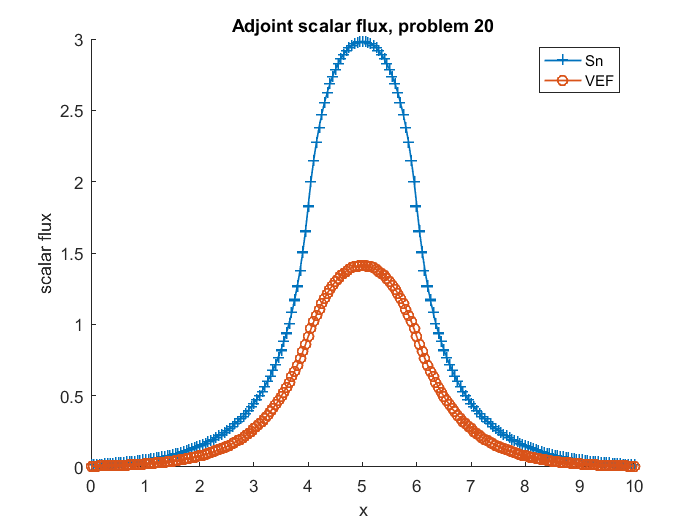
\includegraphics[width=1\linewidth]{p20a.png}
  \caption{Adjoint}
  \label{fig:sub2}
\end{subfigure}
\caption{Unperturbed forward and adjoint solutions for problem 20}
\label{fig:test}
\end{figure}

\subsubsection{Eddington tensor difference}
Below is a graph of the difference in the perturbed and unperturbed Eddington tensor under a $\% 10$ perturbation in $\sigma_t$. The Eddington L1 error for this case is $0.003317$, which is about a 2x increase over case $\#$19, seemingly resulting from the 2x increase in mean free path.
\begin{figure}[H]
\centering
\begin{subfigure}{.5\textwidth}
  \centering
  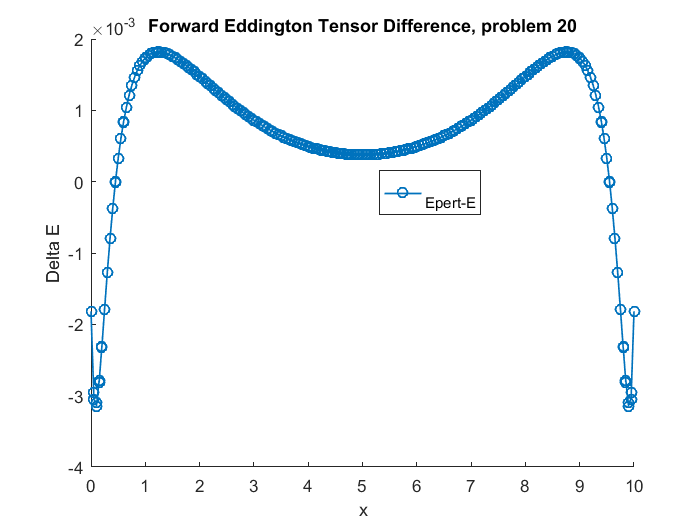
\includegraphics[width=1\linewidth]{p20deltaE.png}
  \caption{$+10\%$ $\sigma_t$. $E_{err}=0.003317$}
  \label{fig:sub1}
\end{subfigure}%
\begin{subfigure}{.5\textwidth}
  \centering
  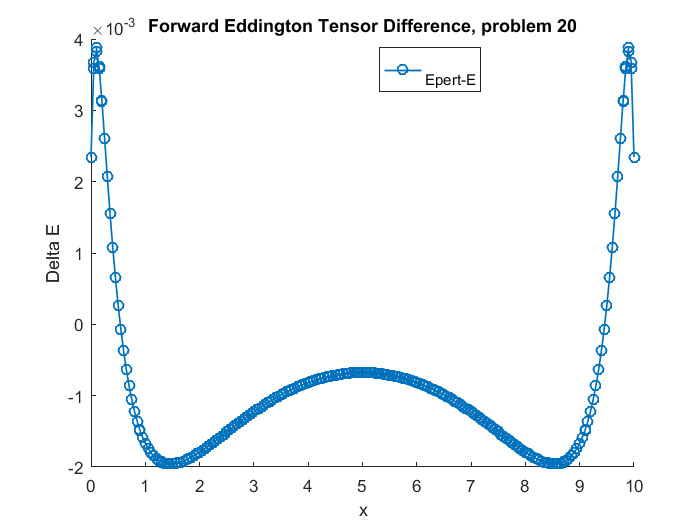
\includegraphics[width=1\linewidth]{p20deltaEdst-10.png}
  \caption{$-10\%$ $\sigma_t$. $E_{err}=0.004170$}
  \label{fig:sub2}
\end{subfigure}
\caption{Eddington difference for $\pm10\%$ $\sigma_t$ for problem 19.}
\label{fig:test}
\end{figure}

\begin{figure}[H]
\centering
\begin{subfigure}{.5\textwidth}
  \centering
  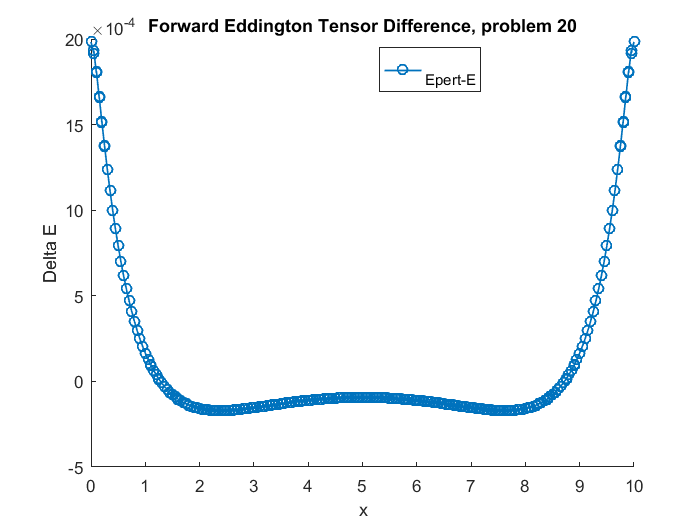
\includegraphics[width=1\linewidth]{p20deltaEdss10.png}
  \caption{$+10\%$ $\sigma_s$. $E_{err}=$}
  \label{fig:sub1}
\end{subfigure}%
\begin{subfigure}{.5\textwidth}
  \centering
  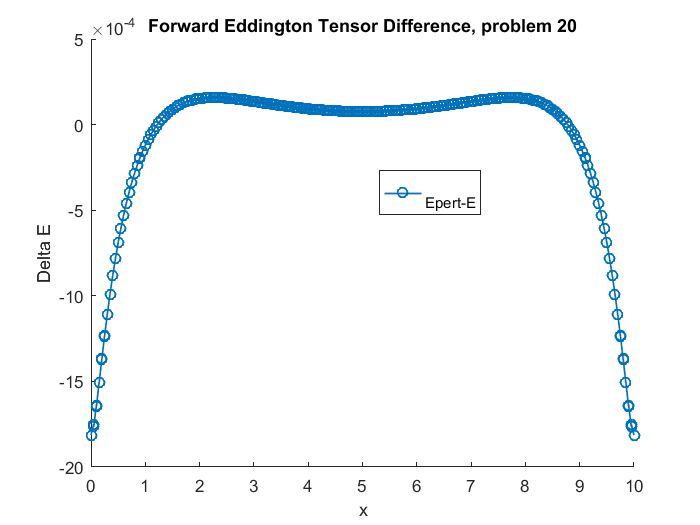
\includegraphics[width=1\linewidth]{p20deltaEdss-10.png}
  \caption{$-10\%$ $\sigma_s$. $E_{err}=$}
  \label{fig:sub2}
\end{subfigure}
\caption{Eddington difference for $\pm10\%$ $\sigma_s$ for problem 20.}
\label{fig:test}
\end{figure}

\begin{figure}[H]
\centering
\begin{subfigure}{.5\textwidth}
  \centering
  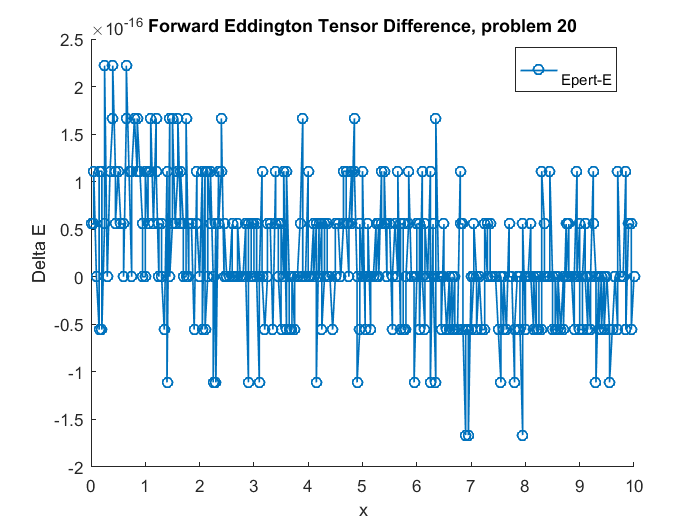
\includegraphics[width=1\linewidth]{p20deltaEdq.png}
  \caption{$+10\%$ $q$. $E_{err}=1.283*10^{-16}$}
  \label{fig:sub1}
\end{subfigure}%
\begin{subfigure}{.5\textwidth}
  \centering
  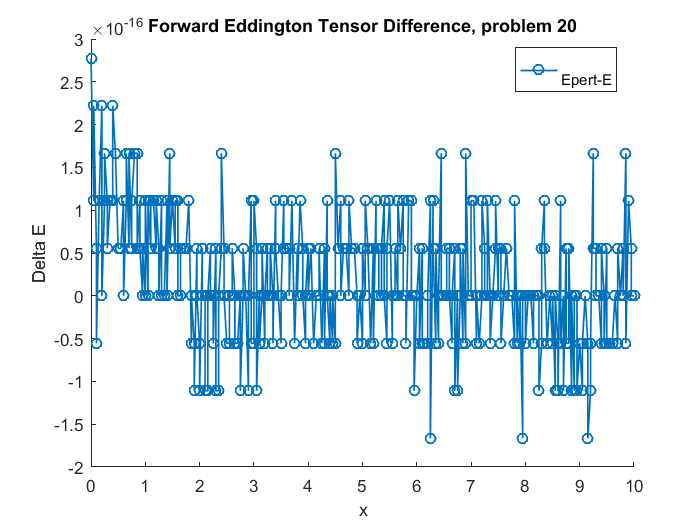
\includegraphics[width=1\linewidth]{p20deltaEdq-10.png}
  \caption{$-10\%$ $q$. $E_{err}=1.412*10^{-16}$}
  \label{fig:sub2}
\end{subfigure}
\caption{Eddington difference for $\pm10\%$ $q$ for problem 19.}
\label{fig:test}
\end{figure}

\begin{figure}[H]
\centering
\begin{subfigure}{.5\textwidth}
  \centering
  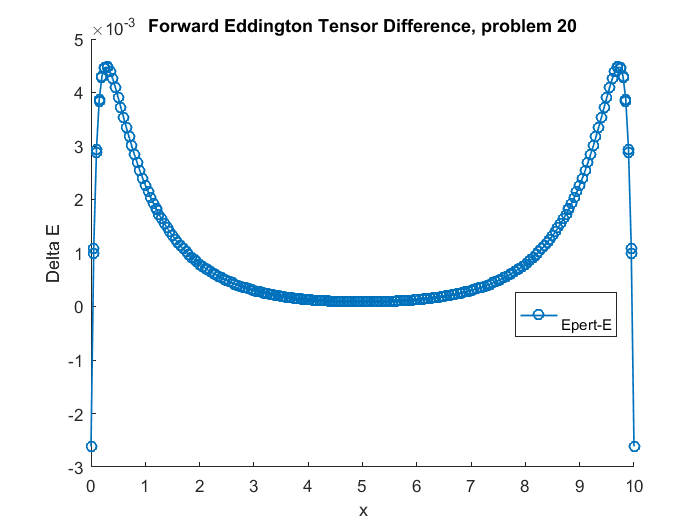
\includegraphics[width=1\linewidth]{p20deltaEdBC0,1.png}
  \caption{$\delta\psi_{inc}=+0.1$. $E_{err}=$}
  \label{fig:sub1}
\end{subfigure}%
\begin{subfigure}{.5\textwidth}
  \centering
  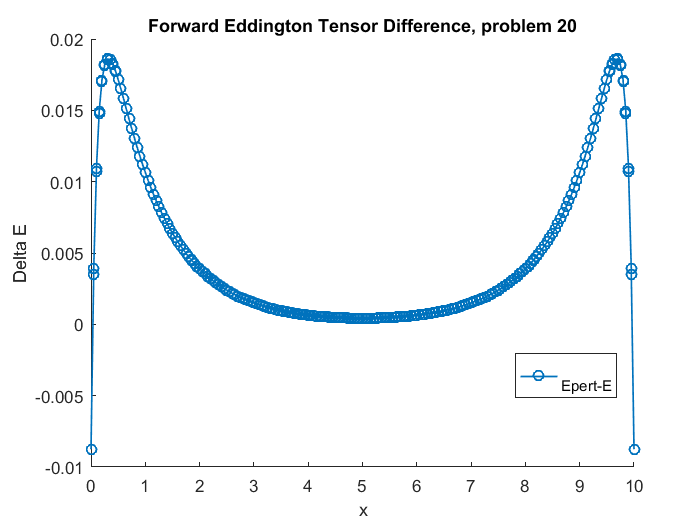
\includegraphics[width=1\linewidth]{p20deltaEdBC0,5.png}
  \caption{$\delta\psi_{inc}=+0.5$. $E_{err}= $}
  \label{fig:sub2}
\end{subfigure}
\caption{Eddington difference for $\psi_{inc}$ perturbations for problem 20.}
\label{fig:test}
\end{figure}

\subsubsection{Perturbation Data Prob 20}
\csvautotabular{DGFEM1D_prob20_short_dst.csv}
\\ \\
\csvautotabular{DGFEM1D_prob20_short_dss.csv}
\\ \\
\csvautotabular{DGFEM1D_prob20_short_dq.csv}
\\ \\
\csvautotabular{DGFEM1D_prob20_short_dBC.csv}

%%%%%%%%%%%%%%%%%%%%%%%%%%%%%%%%%%%%%%%%%%%%%%%%%%%%%%
%%%%%%%%%%%%%%%%%%%%%%%%%%%%%%%%%%%%%%%%%%%%%%%%%%%%%%
\subsection{Case \#21 In load\_input.m}
\subsubsection{Overview}
Further reduction in mean free path from case 19 and 20. Homogeneous region with homogeneous source. No incident flux from either side. Response is sum of flux in middle $1/5$th of region. Region split into 5 zones, each with a width of 2, 40 elements per zone. $\sigma_t = 0.5$ and $\sigma_s=0.25$ for all zones. $\sigma_t$ perturbed uniformly in all zones.

\begin{figure}[H]
\centering
\begin{subfigure}{.5\textwidth}
  \centering
  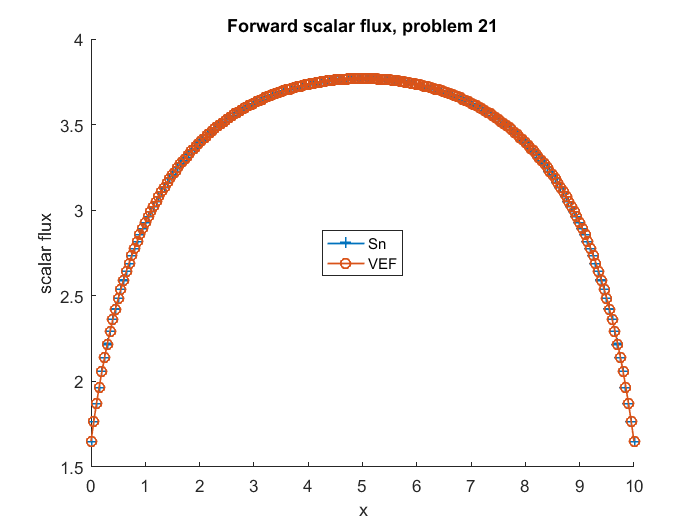
\includegraphics[width=1\linewidth]{p21f.png}
  \caption{Forward}
  \label{fig:sub1}
\end{subfigure}%
\begin{subfigure}{.5\textwidth}
  \centering
  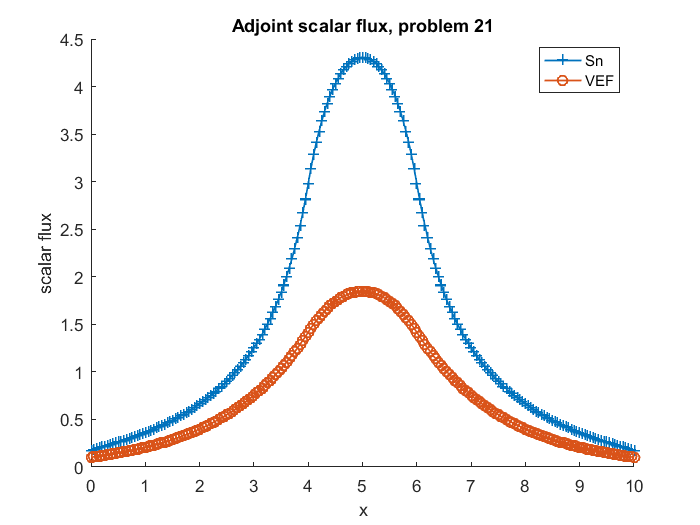
\includegraphics[width=1\linewidth]{p21a.png}
  \caption{Adjoint}
  \label{fig:sub2}
\end{subfigure}
\caption{Unperturbed forward and adjoint solutions for problem 21}
\label{fig:test}
\end{figure}

\subsubsection{Eddington tensor difference}
Below is a graph of the difference in the perturbed and unperturbed Eddington tensor under a $\% 10$ perturbation in $\sigma_t$. The Eddington L1 error for this case is $0.006587$. So, once again we see the 2x increase
\begin{figure}[H]
\centering
\begin{subfigure}{.5\textwidth}
  \centering
  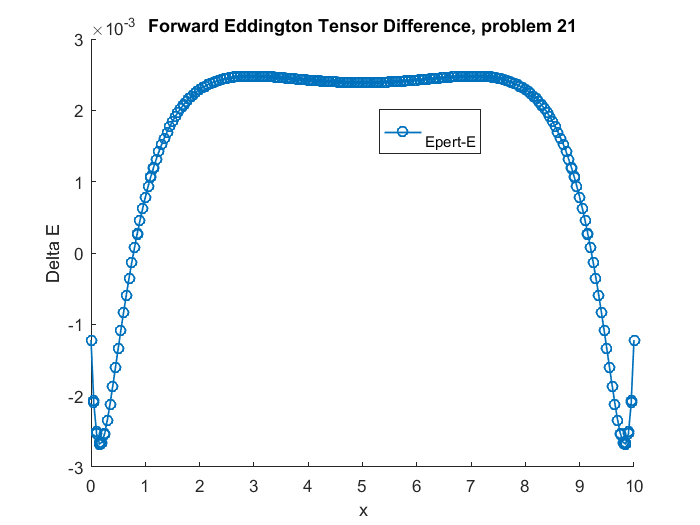
\includegraphics[width=1\linewidth]{p21deltaE.png}
  \caption{$+10\%$ $\sigma_t$. $E_{err}=$}
  \label{fig:sub1}
\end{subfigure}%
\begin{subfigure}{.5\textwidth}
  \centering
  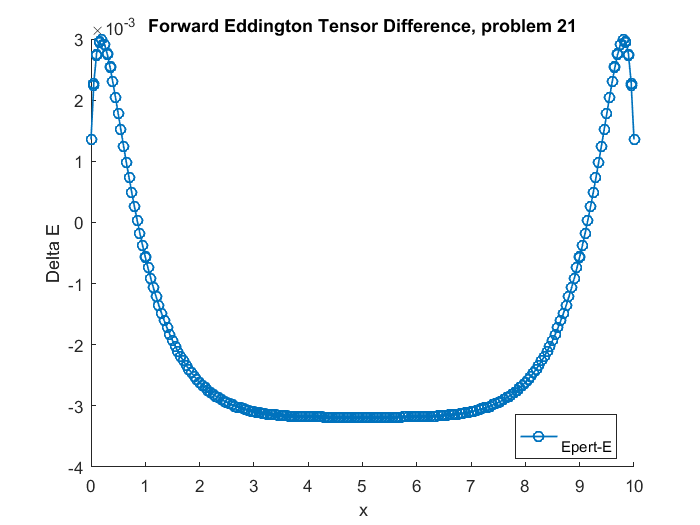
\includegraphics[width=1\linewidth]{p21deltaEdst-10.png}
  \caption{$-10\%$ $\sigma_t$. $E_{err}=$}
  \label{fig:sub2}
\end{subfigure}
\caption{Eddington difference for $\pm$10$\%$ $\sigma_t$ for problem 21.}
\label{fig:test}
\end{figure}

\begin{figure}[H]
\centering
\begin{subfigure}{.5\textwidth}
  \centering
  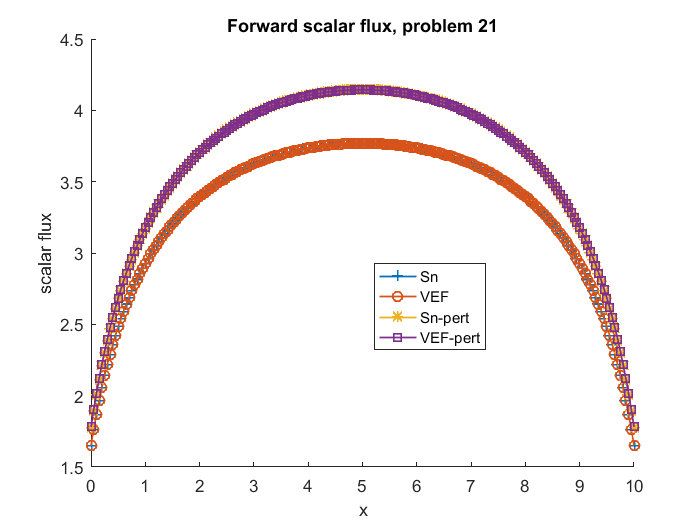
\includegraphics[width=1\linewidth]{p21deltaEdss10.png}
  \caption{$+10\%$ $\sigma_s$. $E_{err}=$}
  \label{fig:sub1}
\end{subfigure}%
\begin{subfigure}{.5\textwidth}
  \centering
  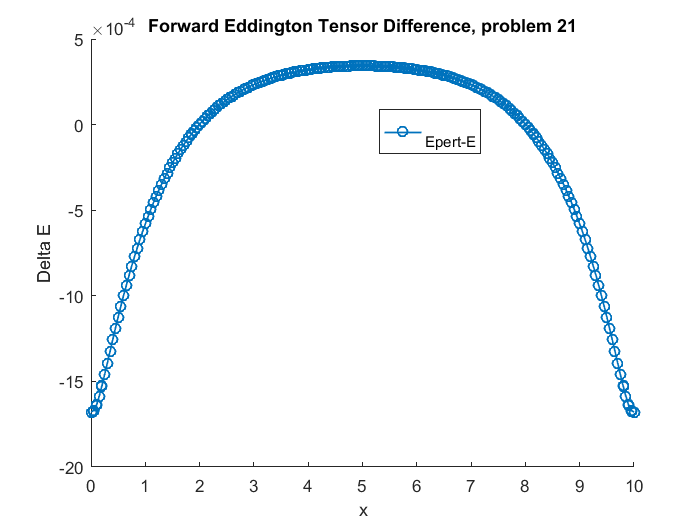
\includegraphics[width=1\linewidth]{p21deltaEdss-10.png}
  \caption{$-10\%$ $\sigma_s$. $E_{err}=$}
  \label{fig:sub2}
\end{subfigure}
\caption{Eddington difference for $\pm10\%$ $\sigma_s$ for problem 21.}
\label{fig:test}
\end{figure}

\begin{figure}[H]
\centering
\begin{subfigure}{.5\textwidth}
  \centering
  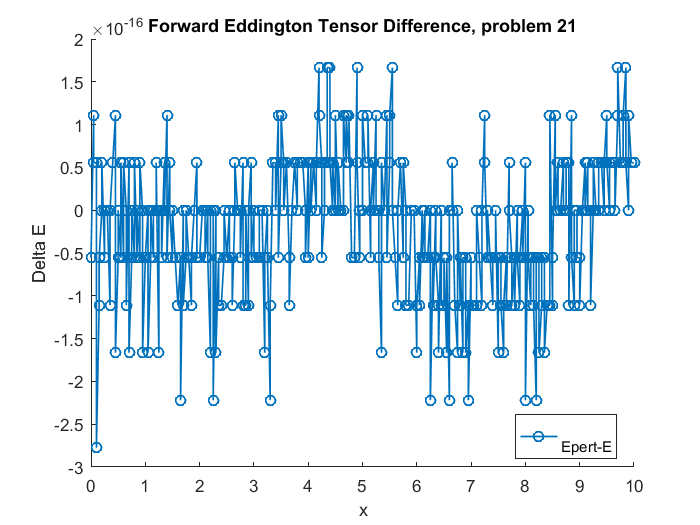
\includegraphics[width=1\linewidth]{p21deltaEdq.png}
  \caption{$+10\%$ $q$. $E_{err}=$}
  \label{fig:sub1}
\end{subfigure}%
\begin{subfigure}{.5\textwidth}
  \centering
  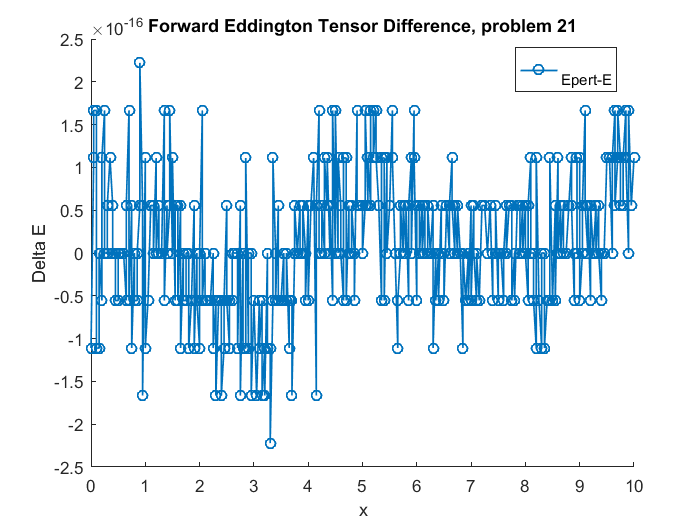
\includegraphics[width=1\linewidth]{p21deltaEdq-10.png}
  \caption{$-10\%$ $q$. $E_{err}=$}
  \label{fig:sub2}
\end{subfigure}
\caption{Eddington difference for $\pm$10$\%$ $q$ for problem 21.}
\label{fig:test}
\end{figure}

\begin{figure}[H]
\centering
\begin{subfigure}{.5\textwidth}
  \centering
  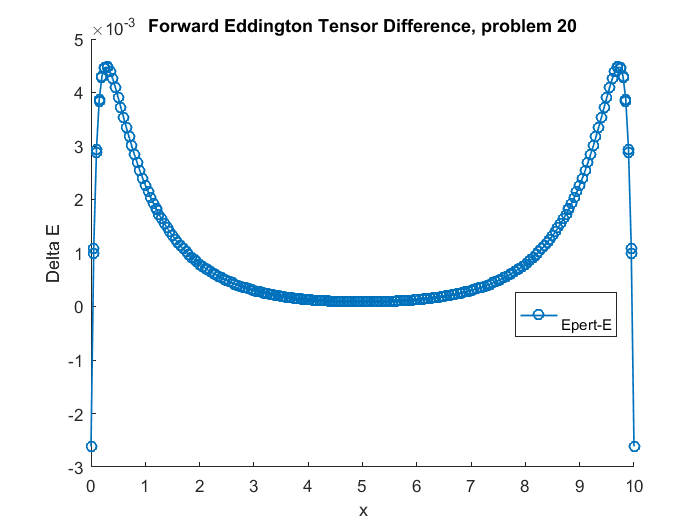
\includegraphics[width=1\linewidth]{p21deltaEdBC0,1.png}
  \caption{$\delta\psi_{inc}=+0.1$. $E_{err}=$}
  \label{fig:sub1}
\end{subfigure}%
\begin{subfigure}{.5\textwidth}
  \centering
  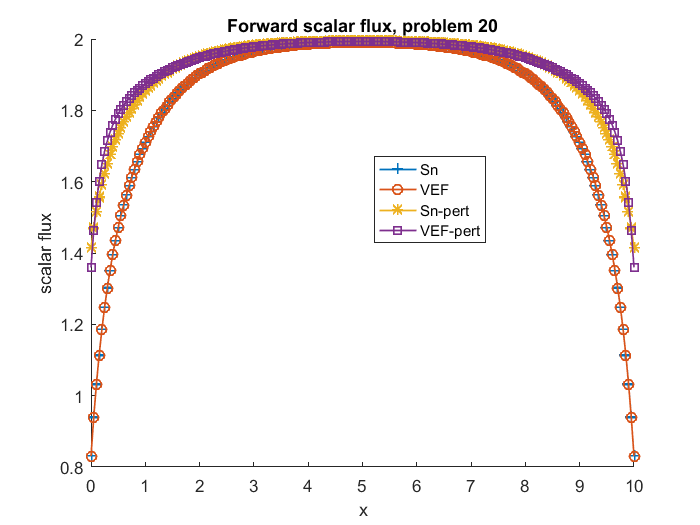
\includegraphics[width=1\linewidth]{p21deltaEdBC0,5.png}
  \caption{$\delta\psi_{inc}=+0.5$. $E_{err}= $}
  \label{fig:sub2}
\end{subfigure}
\caption{Eddington difference for $\psi_{inc}$ perturbations for problem 21.}
\label{fig:test}
\end{figure}

\subsubsection{Perturbation Data Prob 21}
\csvautotabular{DGFEM1D_prob21_short_dst.csv}
\\ \\
\csvautotabular{DGFEM1D_prob21_short_dss.csv}
\\ \\
\csvautotabular{DGFEM1D_prob21_short_dq.csv}
\\ \\
\csvautotabular{DGFEM1D_prob21_short_dBC.csv}

%%%%%%%%%%%%%%%%%%%%%%%%%%%%%%%%%%%%%%%%%%%%%%%%%%%%%
%%%%%%%%%%%%%%%%%%%%%%%%%%%%%%%%%%%%%%%%%%%%%%%%%%%%%
\subsection{Case \#22 In load\_input.m}
\subsubsection{Overview}
Now for something slightly different. Going back to the initial case 19, where $\sigma_t = 2$ and $\sigma_s=1$ for all zones. Now, instead, let us not perturb the first or last 1/5th of the region. These edges are where we see the greatest perturbation in E generally, and by keeping them constant, we may be able to reduce the error due to the perturbed E greatly. 

\begin{figure}[H]
\centering
\begin{subfigure}{.5\textwidth}
  \centering
  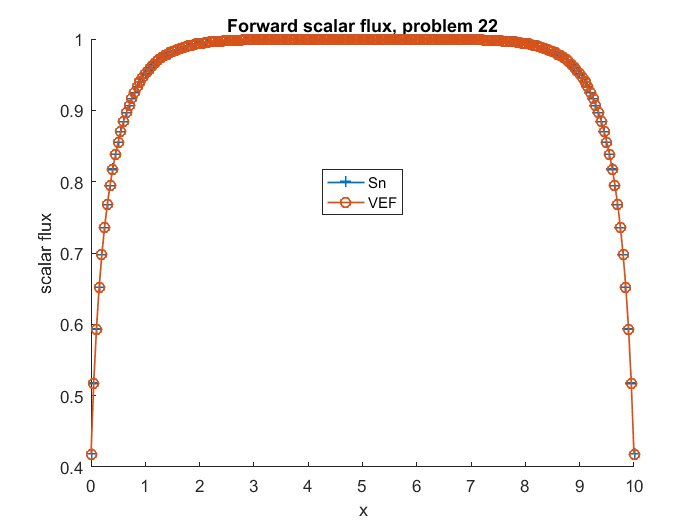
\includegraphics[width=1\linewidth]{p22f.png}
  \caption{Forward}
  \label{fig:sub1}
\end{subfigure}%
\begin{subfigure}{.5\textwidth}
  \centering
  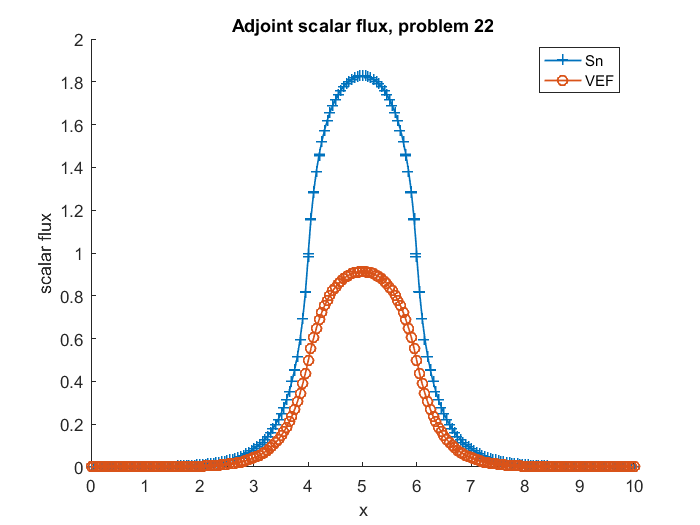
\includegraphics[width=1\linewidth]{p22a.png}
  \caption{Adjoint}
  \label{fig:sub2}
\end{subfigure}
\caption{Unperturbed forward and adjoint solutions for problem 22}
\label{fig:test}
\end{figure}

\subsubsection{Eddington tensor difference}
Graph of the difference in the perturbed and unperturbed Eddington tensor under a $\% 10$ perturbation in $\sigma_t$ only in the middle 3 regions. It's apparent that the Eddington shows the largest perturbation near the boundaries of the problem. The Eddington L1 error for this case is $0.003693$, which is actually greater than the case of uniform perturbation, including the boundary regions.
\begin{figure}[H]
\centering
\begin{subfigure}{.5\textwidth}
  \centering
  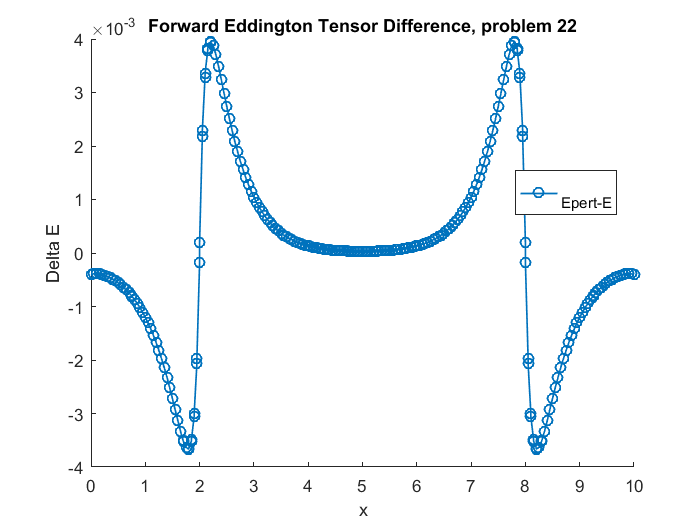
\includegraphics[width=1\linewidth]{p22deltaE.png}
  \caption{$+10\%$ $\sigma_t$. $E_{err}=$}
  \label{fig:sub1}
\end{subfigure}%
\begin{subfigure}{.5\textwidth}
  \centering
  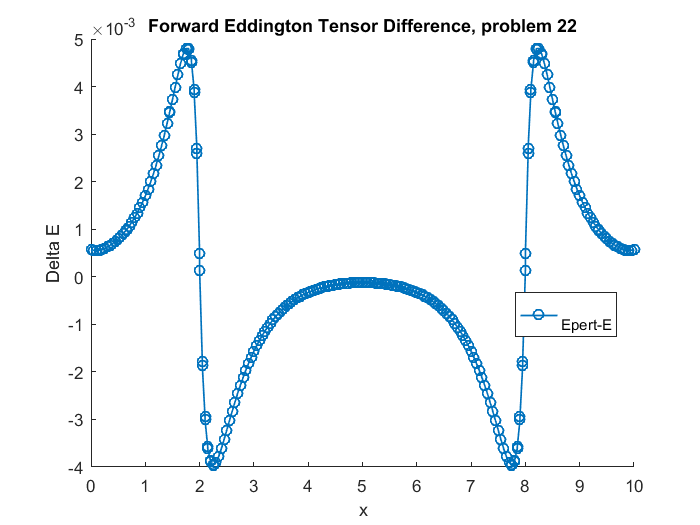
\includegraphics[width=1\linewidth]{p22deltaEdst-10.png}
  \caption{$-10\%$ $\sigma_t$. $E_{err}=$}
  \label{fig:sub2}
\end{subfigure}
\caption{Eddington difference for $\pm$10$\%$ $\sigma_t$ for problem 22.}
\label{fig:test}
\end{figure}

\begin{figure}[H]
\centering
\begin{subfigure}{.5\textwidth}
  \centering
  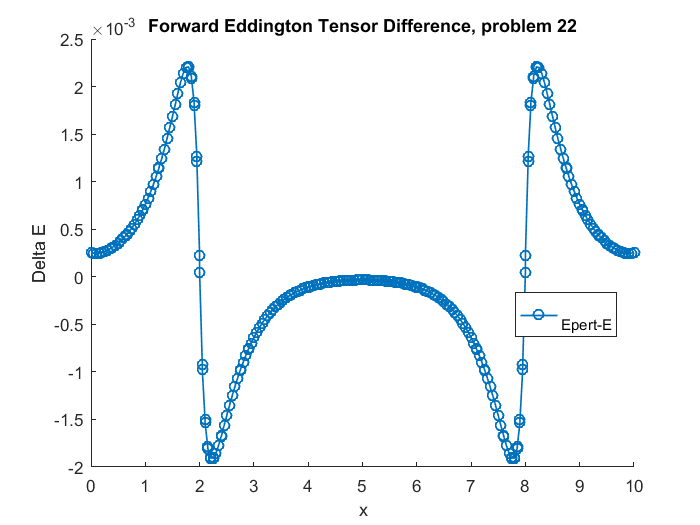
\includegraphics[width=1\linewidth]{p22deltaEdss10.png}
  \caption{$+10\%$ $\sigma_s$. $E_{err}=$}
  \label{fig:sub1}
\end{subfigure}%
\begin{subfigure}{.5\textwidth}
  \centering
  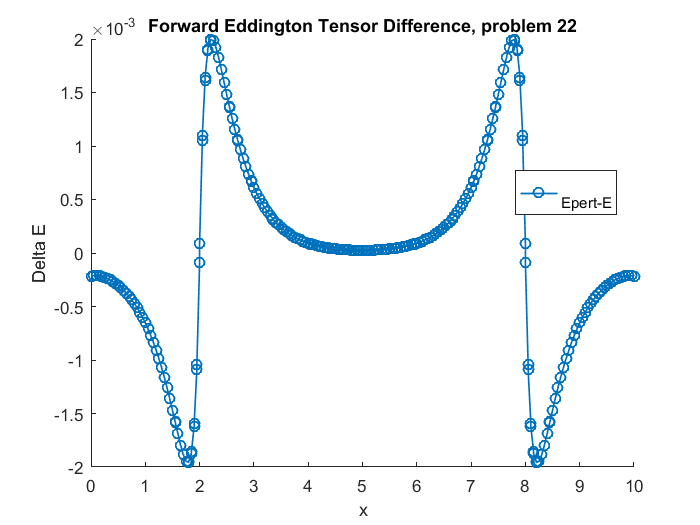
\includegraphics[width=1\linewidth]{p22deltaEdss-10.png}
  \caption{$-10\%$ $\sigma_s$. $E_{err}=$}
  \label{fig:sub2}
\end{subfigure}
\caption{Eddington difference for $\pm10\%$ $\sigma_s$ for problem 22.}
\label{fig:test}
\end{figure}

\begin{figure}[H]
\centering
\begin{subfigure}{.5\textwidth}
  \centering
  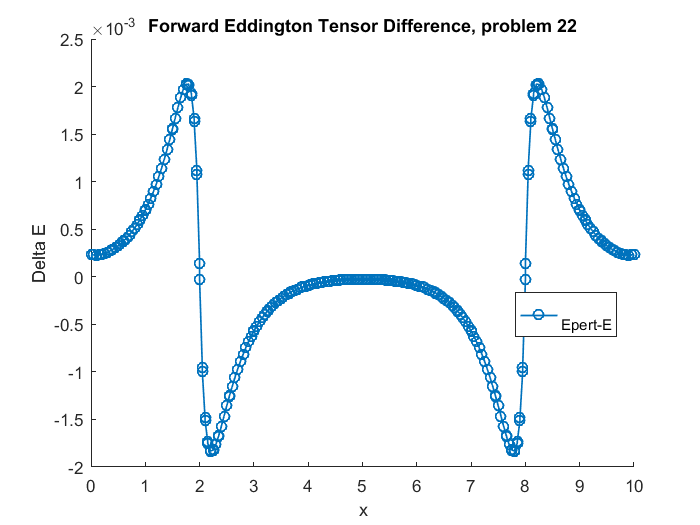
\includegraphics[width=1\linewidth]{p22deltaEdq.png}
  \caption{$+10\%$ $q$. $E_{err}=$}
  \label{fig:sub1}
\end{subfigure}%
\begin{subfigure}{.5\textwidth}
  \centering
  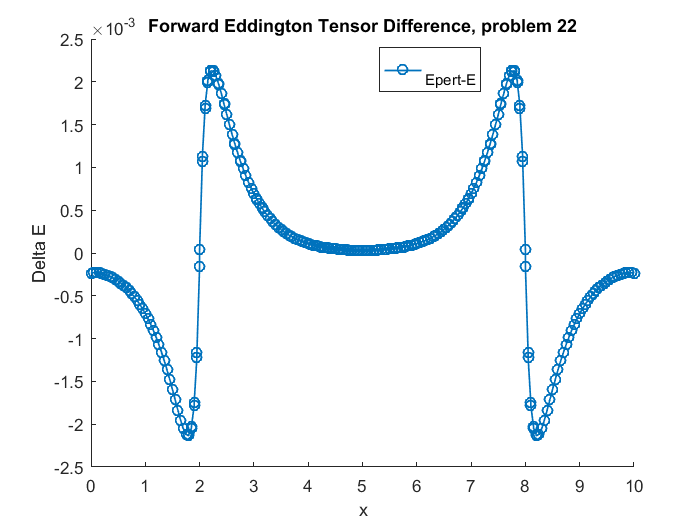
\includegraphics[width=1\linewidth]{p22deltaEdq-10.png}
  \caption{$-10\%$ $q$. $E_{err}=$}
  \label{fig:sub2}
\end{subfigure}
\caption{Eddington difference for $\pm$10$\%$ $q$ for problem 22.}
\label{fig:test}
\end{figure}


\subsubsection{Perturbation Data Prob 22}
\csvautotabular{DGFEM1D_prob22_short_dst.csv}
\\ \\
\csvautotabular{DGFEM1D_prob22_short_dss.csv}
\\ \\
\csvautotabular{DGFEM1D_prob22_short_dq.csv}
\\ \\
\csvautotabular{DGFEM1D_prob22_short_dBC.csv}

%%%%%%%%%%%%%%%%%%%%%%%%%%%%%%%%%%%%%%%%%%%%%%%%%%%%%
%%%%%%%%%%%%%%%%%%%%%%%%%%%%%%%%%%%%%%%%%%%%%%%%%%%%%
\subsection{Case \#23 In load\_input.m}
TODO: Case 20 with no side perts

%%%%%%%%%%%%%%%%%%%%%%%%%%%%%%%%%%%%%%%%%%%%%%%%%%%%%
%%%%%%%%%%%%%%%%%%%%%%%%%%%%%%%%%%%%%%%%%%%%%%%%%%%%%
\subsection{Case \#24 In load\_input.m}
TODO: Case 21 with no side perts

%%%%%%%%%%%%%%%%%%%%%%%%%%%%%%%%%%%%%%%%%%%%%%%%%%%%%
%%%%%%%%%%%%%%%%%%%%%%%%%%%%%%%%%%%%%%%%%%%%%%%%%%%%%
\subsection{Case \#25 In load\_input.m}
Identical to case 19, but with the response on the right boundary 1/5 section.

\begin{figure}[H]
\centering
\begin{subfigure}{.5\textwidth}
  \centering
  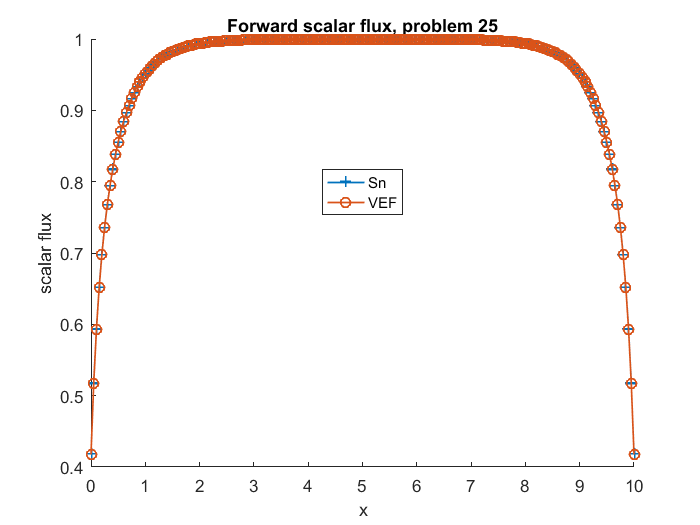
\includegraphics[width=1\linewidth]{p25f.png}
  \caption{Forward}
  \label{fig:sub1}
\end{subfigure}%
\begin{subfigure}{.5\textwidth}
  \centering
  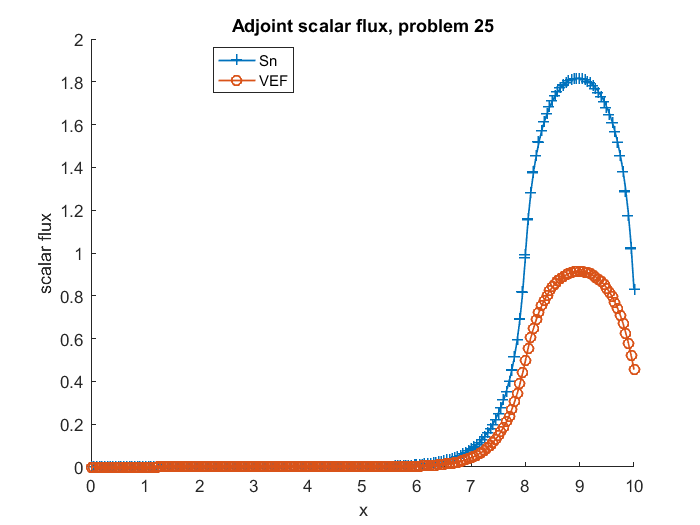
\includegraphics[width=1\linewidth]{p25a.png}
  \caption{Adjoint}
  \label{fig:sub2}
\end{subfigure}
\caption{Unperturbed forward and adjoint solutions for problem 25}
\label{fig:test}
\end{figure}

\subsubsection{Eddington tensor difference}
As expected, same as case 19. Response has no effect on Eddington pert. The Eddington L1 error for this case is $0.001631$
\begin{figure}[H]
\centering
\begin{subfigure}{.5\textwidth}
  \centering
  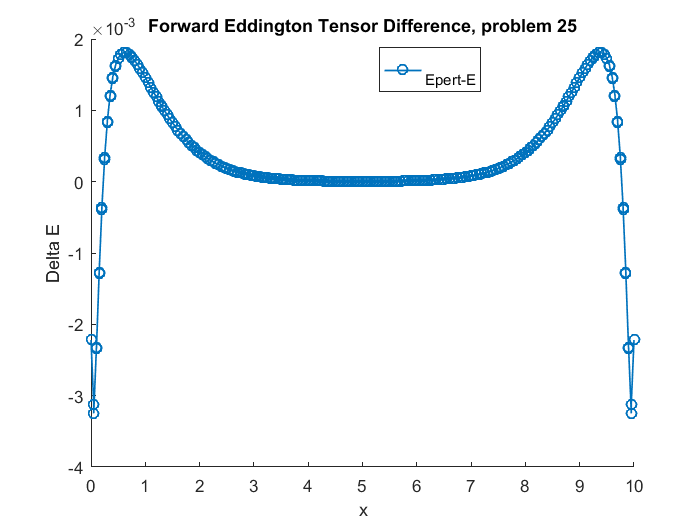
\includegraphics[width=1\linewidth]{p25deltaE.png}
  \caption{$+10\%$ $\sigma_t$. $E_{err}=$}
  \label{fig:sub1}
\end{subfigure}%
\begin{subfigure}{.5\textwidth}
  \centering
  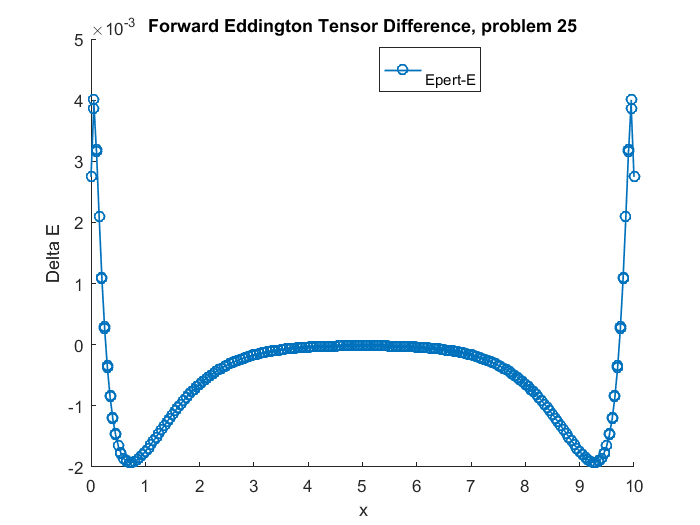
\includegraphics[width=1\linewidth]{p25deltaEdst-10.png}
  \caption{$-10\%$ $\sigma_t$. $E_{err}=$}
  \label{fig:sub2}
\end{subfigure}
\caption{Eddington difference for $\pm$10$\%$ $\sigma_t$ for problem 25.}
\label{fig:test}
\end{figure}

\begin{figure}[H]
\centering
\begin{subfigure}{.5\textwidth}
  \centering
  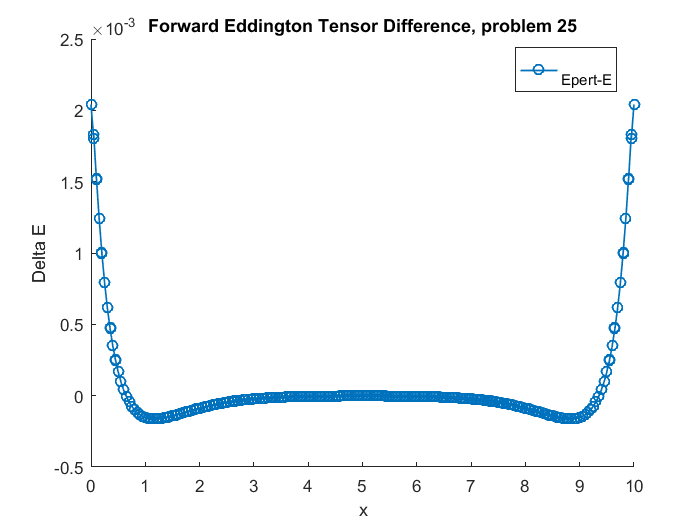
\includegraphics[width=1\linewidth]{p25deltaEdss10.png}
  \caption{$+10\%$ $\sigma_s$. $E_{err}=$}
  \label{fig:sub1}
\end{subfigure}%
\begin{subfigure}{.5\textwidth}
  \centering
  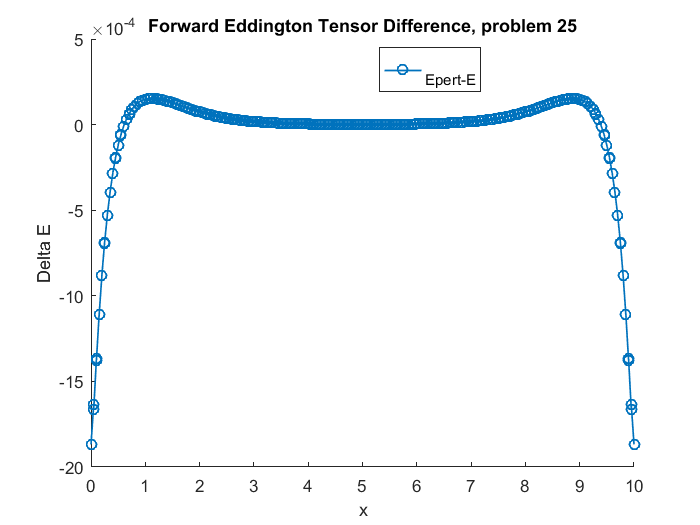
\includegraphics[width=1\linewidth]{p25deltaEdss-10.png}
  \caption{$-10\%$ $\sigma_s$. $E_{err}=$}
  \label{fig:sub2}
\end{subfigure}
\caption{Eddington difference for $\pm10\%$ $\sigma_s$ for problem 25.}
\label{fig:test}
\end{figure}

\begin{figure}[H]
\centering
\begin{subfigure}{.5\textwidth}
  \centering
  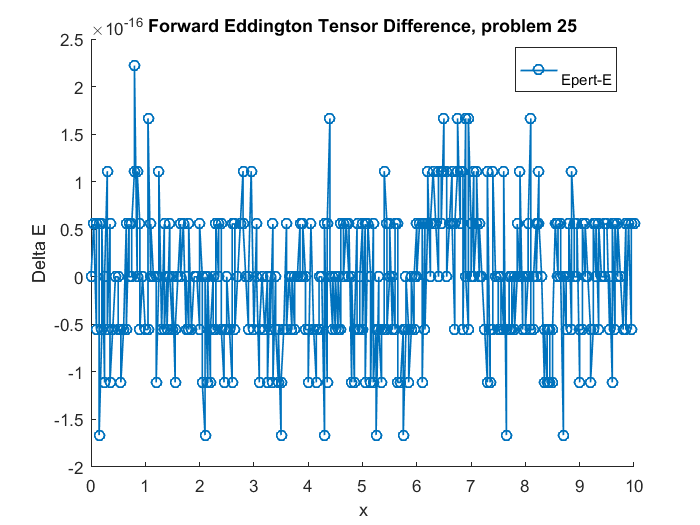
\includegraphics[width=1\linewidth]{p25deltaEdq10.png}
  \caption{$+10\%$ $q$. $E_{err}=$}
  \label{fig:sub1}
\end{subfigure}%
\begin{subfigure}{.5\textwidth}
  \centering
  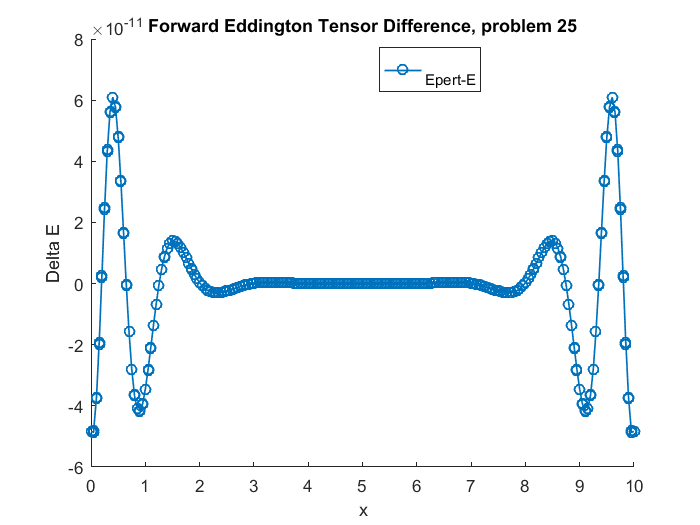
\includegraphics[width=1\linewidth]{p25deltaEdq-10.png}
  \caption{$-10\%$ $q$. $E_{err}=$}
  \label{fig:sub2}
\end{subfigure}
\caption{Eddington difference for $\pm$10$\%$ $q$ for problem 25.}
\label{fig:test}
\end{figure}

\begin{figure}[H]
\centering
\begin{subfigure}{.5\textwidth}
  \centering
  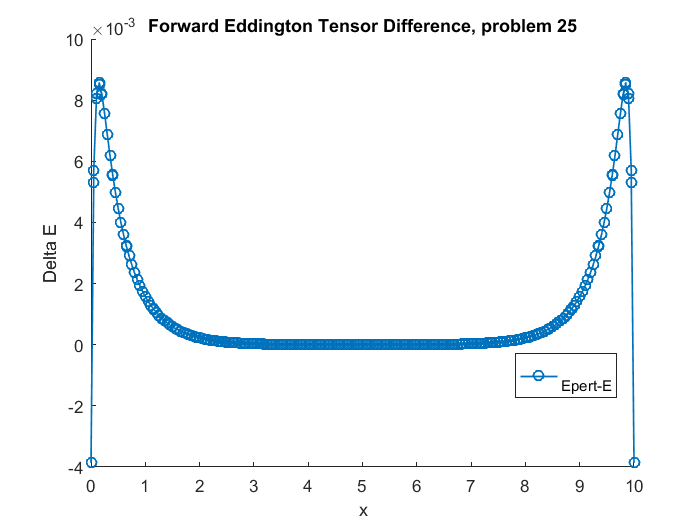
\includegraphics[width=1\linewidth]{p25deltaEdBC0,1.png}
  \caption{$\delta\psi_{inc}=+0.1$. $E_{err}=$}
  \label{fig:sub1}
\end{subfigure}%
\begin{subfigure}{.5\textwidth}
  \centering
  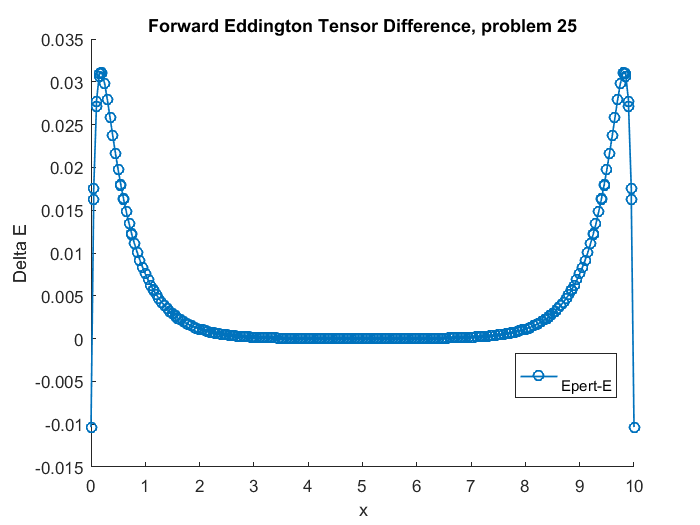
\includegraphics[width=1\linewidth]{p25deltaEdBC0,5.png}
  \caption{$\delta\psi_{inc}=+0.5$. $E_{err}= $}
  \label{fig:sub2}
\end{subfigure}
\caption{Eddington difference for $\psi_{inc}$ perturbations for problem 25.}
\label{fig:test}
\end{figure}

\subsubsection{Perturbation Data Prob 25}
\csvautotabular{DGFEM1D_prob25_short_dst.csv}
\\ \\
\csvautotabular{DGFEM1D_prob25_short_dss.csv}
\\ \\
\csvautotabular{DGFEM1D_prob25_short_dq.csv}
\\ \\
\csvautotabular{DGFEM1D_prob25_short_dBC.csv}

%%%%%%%%%%%%%%%%%%%%%%%%%%%%%%%%%%%%%%%%%%%%%%%%%%%%%%%%%%
\section{Some test case comparisons. $\Sigma_t$ pert}
%%%%%%%%%%%%%%%%%%%%%%%%%%%%%%%%%%%%%%%%%%%%%%%%%%%%%%%%%%
\subsection{Increasing mfp}
\begin{align*}
&\text{Case 19} \to \Sigma_t=2, \Sigma_s=1 \\
&\text{Case 20} \to \Sigma_t=1, \Sigma_s=0.5 \\
&\text{Case 21} \to \Sigma_t=0.5, \Sigma_s=0.25 
\end{align*}
\begin{figure}[H]
\centering
\begin{subfigure}{.49\textwidth}
  \centering
  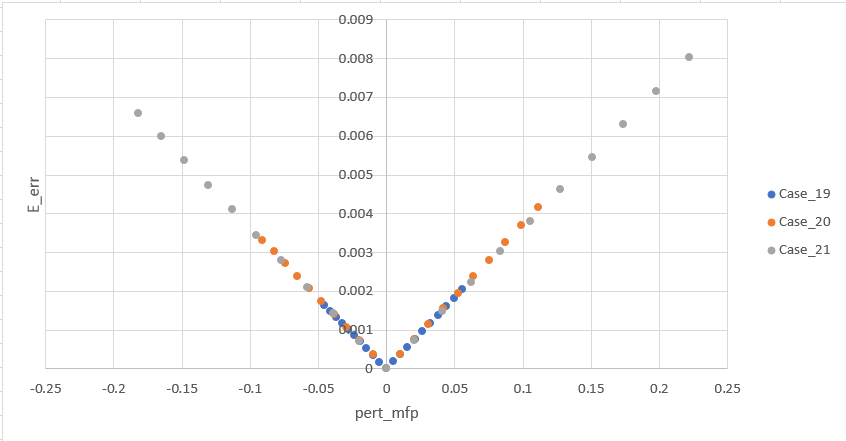
\includegraphics[width=1\linewidth]{EerrVsMfp1.png}
  \caption{$E_{err}$ vs $\delta mfp$}
  \label{fig:sub1}
\end{subfigure}%
\begin{subfigure}{.49\textwidth}
  \centering
  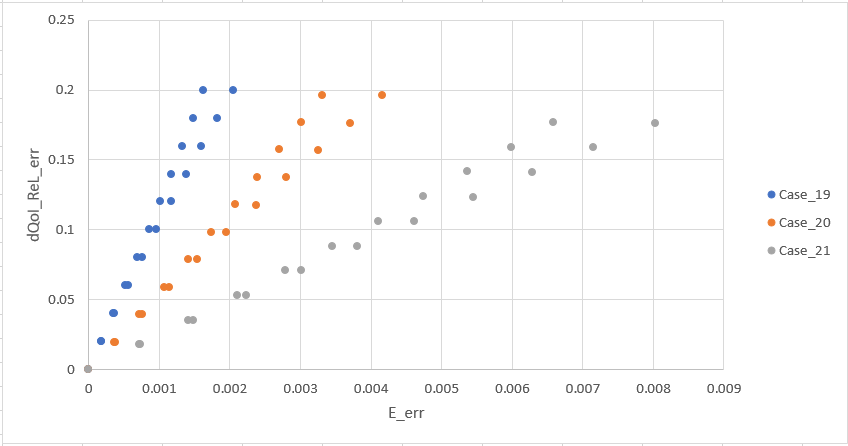
\includegraphics[width=1\linewidth]{dQOIVsEerr1.png}
  \caption{$\delta QoI_{err}$ vs $E_{err}$}
  \label{fig:sub2}
\end{subfigure}
\vskip\baselineskip
\begin{subfigure}{.49\textwidth}
  \centering
  \includegraphics[width=1\linewidth]{dQOIVsMfp1.png}
  \caption{$\delta QoI_{err}$ vs $\delta mfp$}
  \label{fig:sub3}
\end{subfigure}
\begin{subfigure}{.49\textwidth}
  \centering
  \includegraphics[width=1\linewidth]{dQOIdivMfpVsSiga1.png}
  \caption{$\delta QoI_{err}/\delta mfp$ vs $\sigma_{a,pert}$}
  \label{fig:sub4}
\end{subfigure}
\caption{Various relations under increasing mean free path. Problems 19,20,21.}
\label{fig:Comp1}
\end{figure}

\subsection{Reduced pert regions}
\begin{align*}
&\text{Case 19} \to \text{Full region pert} \\
&\text{Case 22} \to \text{Mid 3/5 pert} \\
\end{align*}
\begin{figure}[H]
\centering
\begin{subfigure}{.49\textwidth}
  \centering
  \includegraphics[width=1\linewidth]{EerrVsMfp2.png}
  \caption{$E_{err}$ vs $\delta mfp$}
  \label{fig:sub1}
\end{subfigure}%
\begin{subfigure}{.49\textwidth}
  \centering
  \includegraphics[width=1\linewidth]{dQOIVsEerr2.png}
  \caption{$\delta QoI_{err}$ vs $E_{err}$}
  \label{fig:sub2}
\end{subfigure}
\vskip\baselineskip
\begin{subfigure}{.49\textwidth}
  \centering
  \includegraphics[width=1\linewidth]{dQOIVsMfp2.png}
  \caption{$\delta QoI_{err}$ vs $\delta mfp$}
  \label{fig:sub3}
\end{subfigure}
\begin{subfigure}{.49\textwidth}
  \centering
  \includegraphics[width=1\linewidth]{dQOIdivMfpVsSiga2.png}
  \caption{$\delta QoI_{err}/\delta mfp$ vs $\sigma_{a,pert}$}
  \label{fig:sub4}
\end{subfigure}
\caption{Various relations under reduced perturbation regions. Problems 19 and 22.}
\label{fig:Comp1}
\end{figure}

\subsection{Changes to $\sigma_s$}
\begin{align*}
&\text{Case 19} \to \Sigma_t=2, \Sigma_s=1 \\
&\text{Case 20} \to \Sigma_t=2, \Sigma_s=1.1\\
&\text{Case 21} \to \Sigma_t=2, \Sigma_s=0.9
\end{align*}
\begin{figure}[H]
\centering
\begin{subfigure}{.49\textwidth}
  \centering
  \includegraphics[width=1\linewidth]{EerrVsMfp3.png}
  \caption{$E_{err}$ vs $\delta mfp$}
  \label{fig:sub1}
\end{subfigure}%
\begin{subfigure}{.49\textwidth}
  \centering
  \includegraphics[width=1\linewidth]{dQOIVsEerr3.png}
  \caption{$\delta QoI_{err}$ vs $E_{err}$}
  \label{fig:sub2}
\end{subfigure}
\vskip\baselineskip
\begin{subfigure}{.49\textwidth}
  \centering
  \includegraphics[width=1\linewidth]{dQOIVsMfp3.png}
  \caption{$\delta QoI_{err}$ vs $\delta mfp$}
  \label{fig:sub3}
\end{subfigure}
\begin{subfigure}{.49\textwidth}
  \centering
  \includegraphics[width=1\linewidth]{dQOIdivMfpVsSiga3.png}
  \caption{$\delta QoI_{err}/\delta mfp$ vs $\sigma_{a,pert}$}
  \label{fig:sub4}
\end{subfigure}
\caption{Various relations under changes to $\Sigma_s$ values. Problems 19, 27, 28.}
\label{fig:Comp1}
\end{figure}

%%%%%%%%%%%%%%%%%%%%%%%%%%%%%%%%%%%%%%%%%%%%%%%%%%%%%%%%%%
\section{Some test case comparisons. $\Sigma_s$ pert}
%%%%%%%%%%%%%%%%%%%%%%%%%%%%%%%%%%%%%%%%%%%%%%%%%%%%%%%%%%
\subsection{Increasing mfp}
\begin{align*}
&\text{Case 19} \to \Sigma_t=2, \Sigma_s=1 \\
&\text{Case 20} \to \Sigma_t=1, \Sigma_s=0.5 \\
&\text{Case 21} \to \Sigma_t=0.5, \Sigma_s=0.25 
\end{align*}
\begin{figure}[H]
\centering
\begin{subfigure}{.49\textwidth}
  \centering
  \includegraphics[width=1\linewidth]{EerrVsMfp4.png}
  \caption{$E_{err}$ vs $\delta smfp$}
  \label{fig:sub1}
\end{subfigure}%
\begin{subfigure}{.49\textwidth}
  \centering
  \includegraphics[width=1\linewidth]{dQOIVsEerr4.png}
  \caption{$\delta QoI_{err}$ vs $E_{err}$}
  \label{fig:sub2}
\end{subfigure}
\vskip\baselineskip
\begin{subfigure}{.49\textwidth}
  \centering
  \includegraphics[width=1\linewidth]{dQOIVsMfp4.png}
  \caption{$\delta QoI_{err}$ vs $\delta smfp$}
  \label{fig:sub3}
\end{subfigure}
\begin{subfigure}{.49\textwidth}
  \centering
  \includegraphics[width=1\linewidth]{dQOIdivMfpVsSiga4.png}
  \caption{$\delta QoI_{err}/\delta smfp$ vs $\sigma_{a,pert}$}
  \label{fig:sub4}
\end{subfigure}
\caption{Various relations under increasing mean free path. Problems 19,20,21.}
\label{fig:Comp1}
\end{figure}

\subsection{Reduced pert regions}
\begin{align*}
&\text{Case 19} \to \text{Full region pert} \\
&\text{Case 22} \to \text{Mid 3/5 pert} \\
\end{align*}


\newpage

\textbf{This document was created using \LaTeX}

\end{document}
